\section{Results}\label{sec:results}

The comparative analysis revealed that \ac{rpm} outperformed \ac{sog} 
as a predictor of fuel consumption in the baseline model. 
This finding is supported both empirically (as shown by higher R² values and lower prediction errors) 
and theoretically by the fundamental mechanics of marine propulsion systems.
Specifically, \ac{rpm} is directly linked to the engine's rotational workload and thus 
to power output and fuel consumption, which often follows a cubic or higher-order nonlinear relationship 
with shaft speed \cite{alireza2018fuelengine}. 
In contrast, \ac{sog} is a kinematic parameter influenced by environmental forces such as wind, currents, 
and tides, which decouple it from the actual engine load and energy usage.

Linear and simpler models tend to outperform complex and non-linear ones. This is demonstrated in \cref{tab:baseline_model_cross_validation}. The table presents the baseline performance metrics of four regression models—Ridge Regression, Support Vector Regression (SVR), Random Forest, and XGBoost—evaluated using five-fold cross-validation. The comparison includes the mean and standard deviation of R², adjusted R², RMSE (Root Mean Squared Error), and MAE (Mean Absolute Error), offering a robust assessment of both model accuracy and consistency. Among the evaluated models, Ridge Regression outperforms the others, achieving the highest mean R² (0.7606) and adjusted R² (0.7597) values, indicating a stronger explanatory power with minimal overfitting. It also attains the lowest average RMSE (5.9762) and MAE (3.1582), suggesting superior predictive accuracy and lower average error in fuel consumption estimation. SVR ranks second across most metrics, with a slightly lower R² (0.7261) and adjusted R² (0.7251), along with a higher RMSE (6.4549) and MAE (3.3779), indicating moderately reduced performance relative to Ridge Regression. Random Forest performs worse than both Ridge and SVR, particularly in terms of error metrics, while XGBoost shows the lowest performance overall, with the smallest R² (0.6062) and highest RMSE (7.6537) and MAE (4.1084), indicating less effective generalization to the data. In terms of variability, all models demonstrate comparable standard deviations across folds, with Ridge Regression maintaining the lowest variance in both RMSE and MAE, underscoring its reliability and stability.

Feature analysis revealed that adding environment variables proved beneficial in predicting FC compared to baseline as shown in \cref{tab:advanced_model_cross_validation}. Among the evaluated models, Random Forest yields the best overall performance, achieving the highest mean R² (0.9021) and adjusted R² (0.9006), indicating superior explanatory power. It also records the lowest RMSE (3.5385) and MAE (2.1864), underscoring its high predictive accuracy and minimal average deviation between predicted and actual fuel consumption values. Additionally, the relatively low standard deviations across folds highlight the model’s consistency. Ridge Regression, XGBoost, and SVR exhibit comparable predictive performance, with R² values ranging from 0.8906 to 0.8941 and similar RMSE values (~3.71 for Ridge and XGBoost; 3.64 for SVR). However, SVR attains a slightly higher adjusted R² (0.8925) than Ridge and XGBoost and shows a lower MAE than both, suggesting that SVR may yield marginally better performance in minimizing absolute prediction errors with slightly greater variability across folds (MAE std: 0.4149). Overall, the results underscore that ensemble-based methods like Random Forest are particularly effective in modeling fuel consumption when more advanced modeling strategies are employed. The transition from baseline to advanced models led to a significant improvement in predictive performance across all metrics. In the baseline setup, Ridge Regression performed best, but in the advanced configuration, Random Forest emerged as the top performer with a notable increase in R² (from 0.76 to 0.90) and substantial reductions in RMSE and MAE. These improvements reflect enhanced model accuracy, better generalization, and increased stability.

Most influencial parameters that contributed significantly to the overall accuracy and were used in building the advanced model in the order of importance are Engine RPM, Temperature in surface snow, seawater salinity, and Propeller slip. All other features contributed somewhat but needed to be more significant to justify their usage in the final model, and therefore, they were not used. These findings are depicted in \cref{fig:random_forest_tree,fig:features_importance}. The bar plot presents the feature importance scores derived from a tree-based model Random Forest, used for predicting fuel consumption. The feature importance metric reflects the contribution of each input variable to reducing the prediction error, and hence to the overall model performance. In order to not skew the figure the Engine RPM have been filtered out from the view. The most influential features are "tsn", "tsr", and "spd", each exhibiting the highest importance scores and their dominant contribution emphasizes the critical role of environment-related metrics in determining fuel consumption. Following these are meteorological and geospatial variables such as "mssl", "mstp", and "longitude", along with temporal features like "day" and "wo" (week of observation). This indicates that, beyond machinery metrics, environmental conditions and voyage context also play a non-negligible role in shaping fuel use dynamics. Several oceanographic and weather-related parameters (e.g., "p140208", "ppbd", "mwd", "mwsh") fall into a mid-importance range, suggesting their secondary influence on consumption, potentially through effects on vessel resistance or route adjustments. Conversely, the features toward the right end of the plot (e.g., "sicom", "sige", "ssmtbkc") exhibit minimal importance, implying limited predictive value in the current modeling setup.

\begin{figure}[htbp]
    \centering
        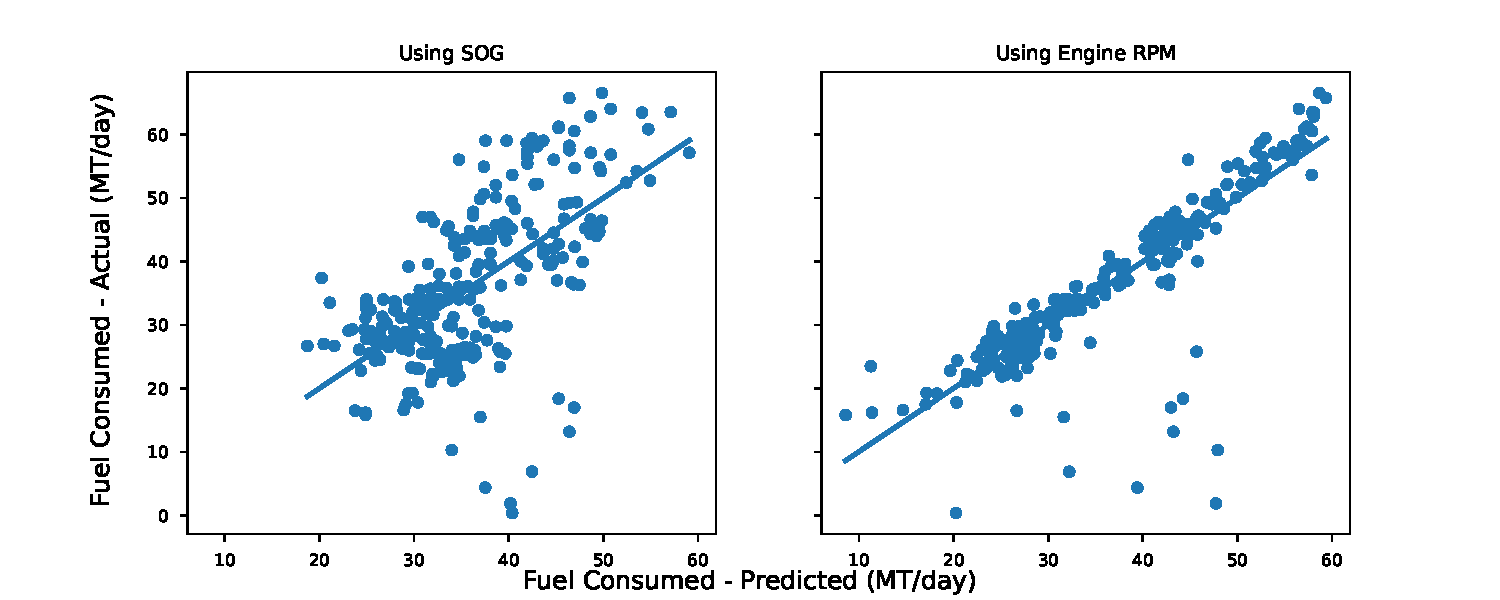
\includegraphics[width=1\textwidth]{sog_vs_engine_rpm_using_ridge.pdf}
        \caption[Baseline Ridge to Compare Fit]{SOG vs Engine RPM}
        \label{fig:baseline_ridge_to_compare_fit_using_sog_vs_engine_rpm}
\end{figure}

\begin{figure}[htbp]
    \centering
    \includegraphics[width=\linewidth]{random_forest_tree.pdf}
    \caption{Random Forest Tree}
    \label{fig:random_forest_tree}
\end{figure}

\begin{figure}[htbp]
    \centering
        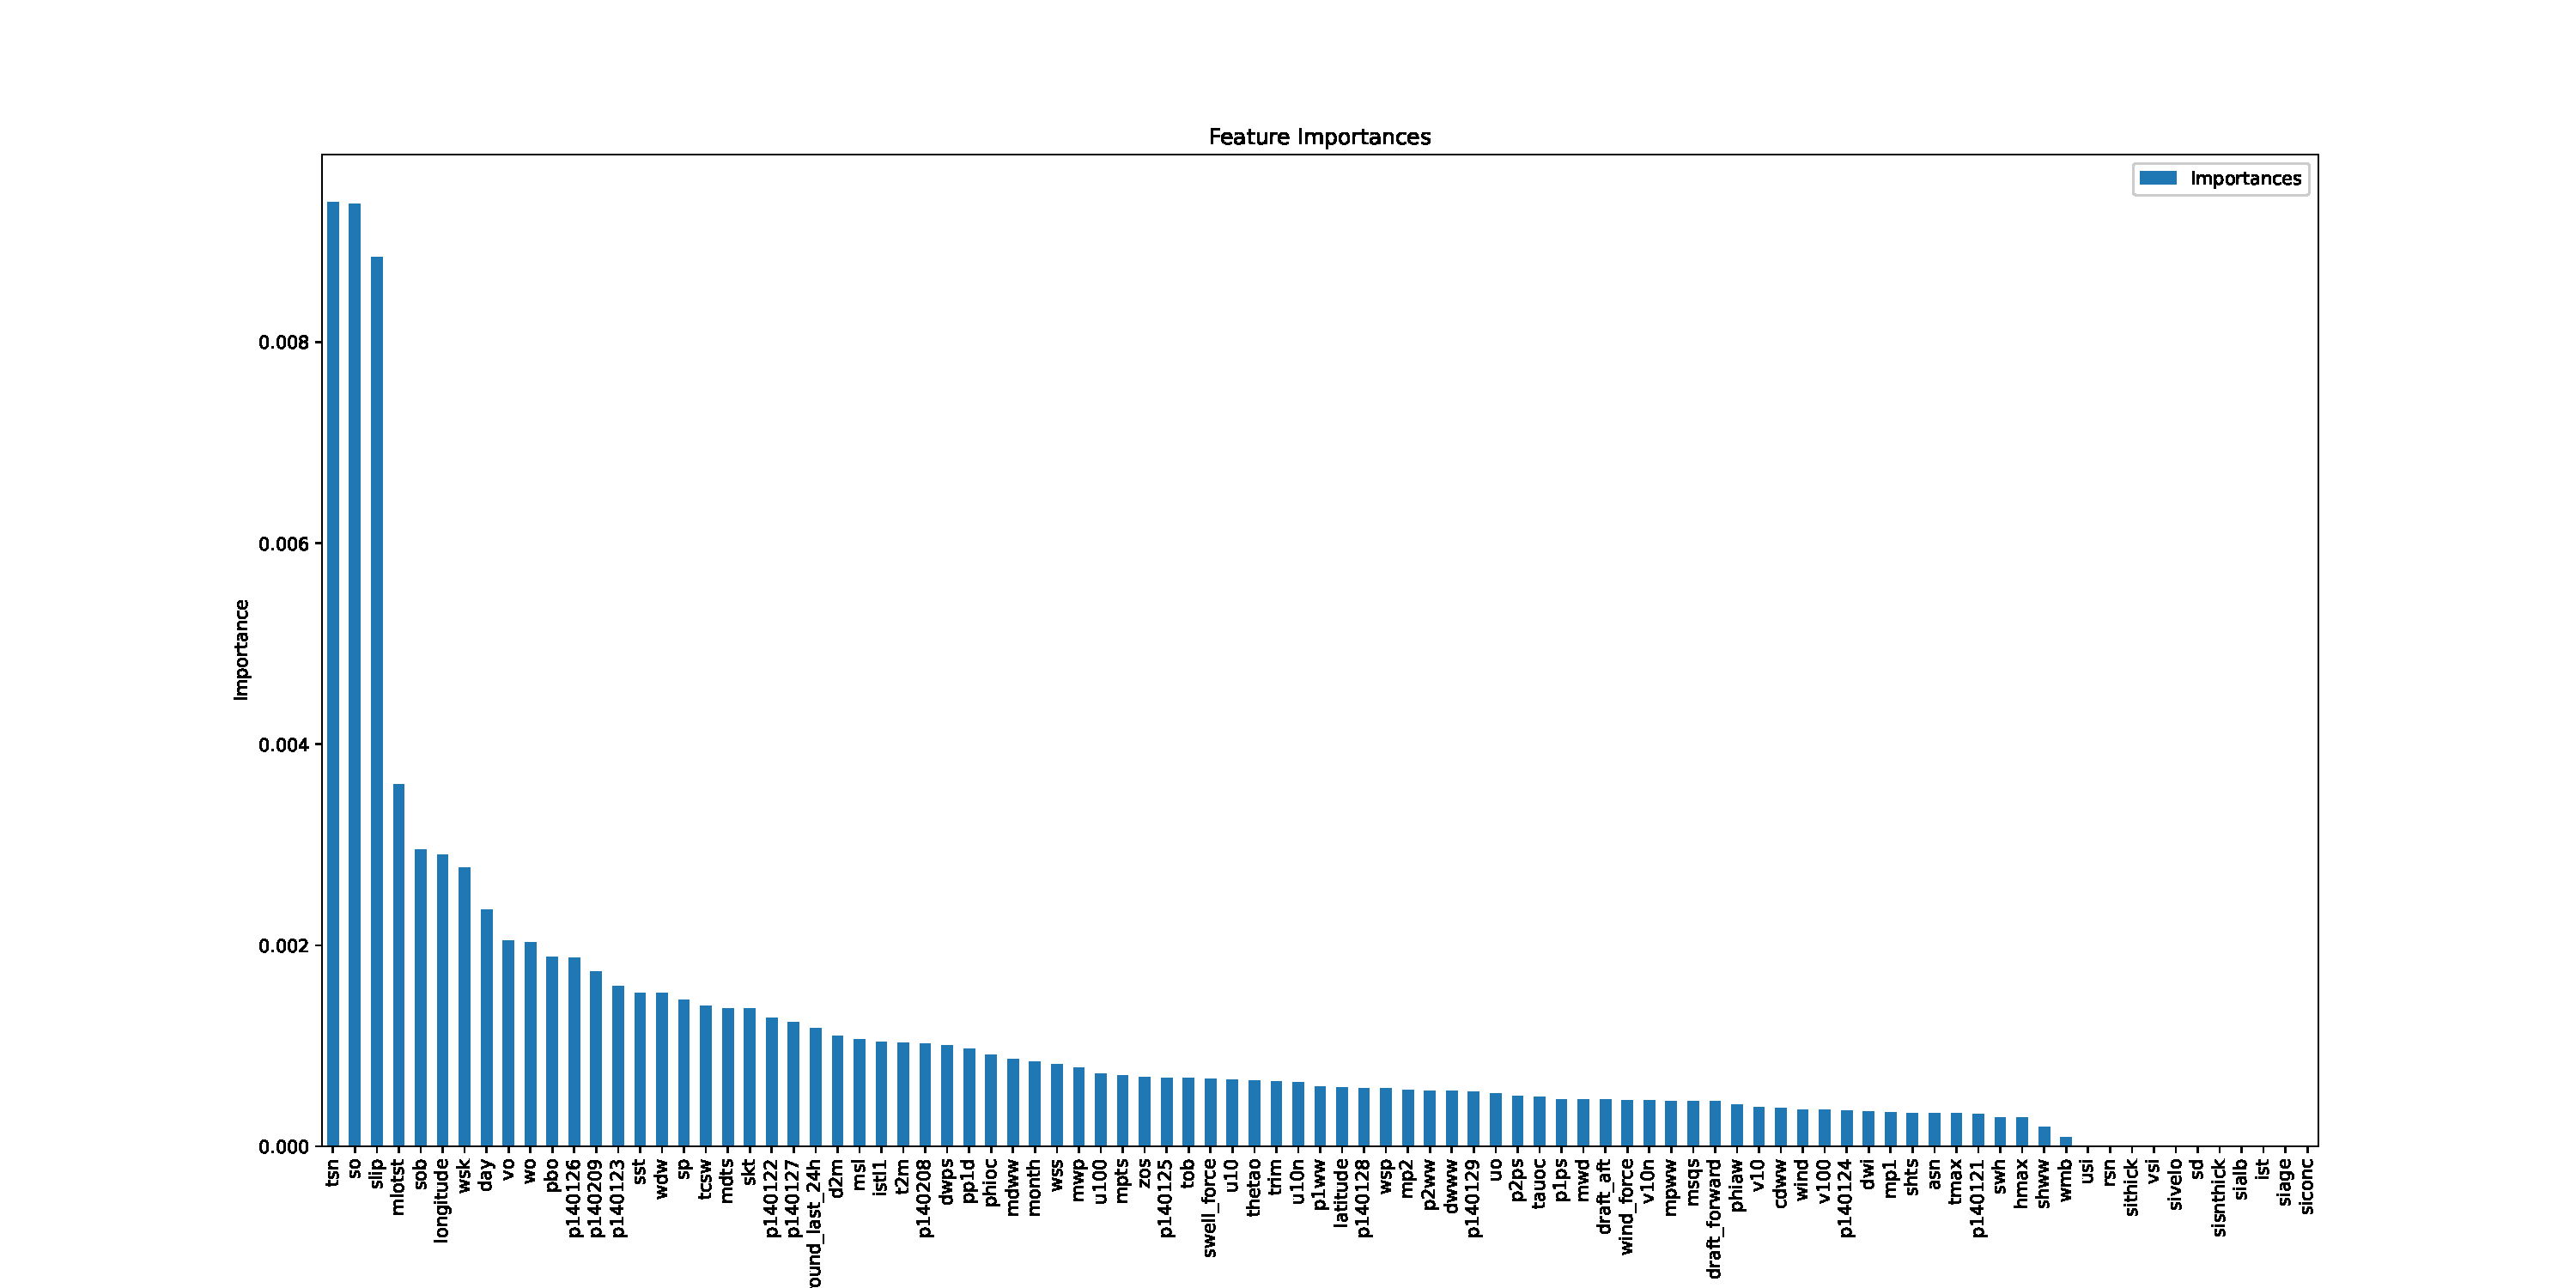
\includegraphics[width=1\textwidth]{features_importance.pdf}
        \caption[Features Importance]{Excluding Engine RPM}
        \label{fig:features_importance}
\end{figure}


\begin{table}[!ht]
        \centering
        \caption{Baseline Performance Comparison with Five Fold Cross}
        \resizebox{\textwidth}{!}{%
        \begin{tabular}{lrrrrrrrr}
        \toprule
        {} &   \textbf{r2\_mean} &    \textbf{r2\_std} &  \textbf{adj\_r2\_mean} &  \textbf{adj\_r2\_std} &  \textbf{rmse\_mean} &  \textbf{rmse\_std} &  \textbf{mae\_mean} &   \textbf{mae\_std} \\
        \midrule
        ridge        &  0.760612 &  0.130927 &     0.759735 &    0.131407 &   5.976210 &  2.002627 &  3.158223 &  0.734065 \\
        svr          &  0.726106 &  0.126659 &     0.725103 &    0.127123 &   6.454855 &  1.918580 &  3.377862 &  0.832788 \\
        randomforest &  0.690246 &  0.138696 &     0.689111 &    0.139204 &   6.792727 &  2.029012 &  3.710294 &  0.712134 \\
        xgboost      &  0.606152 &  0.162200 &     0.604709 &    0.162794 &   7.653745 &  2.014358 &  4.108379 &  0.774200 \\
        \bottomrule
        \end{tabular}%
        }
        \label{tab:baseline_model_cross_validation}
\end{table}
\begin{table}[!ht]
        \centering
        \caption{Advanced Model Performance Comparison with Five Fold Cross}
        \resizebox{\textwidth}{!}{%
        \begin{tabular}{lrrrrrrrr}
        \toprule
        {} &   \textbf{r2\_mean} &    \textbf{r2\_std} &  \textbf{adj\_r2\_mean} &  \textbf{adj\_r2\_std} &  \textbf{rmse\_mean} &  \textbf{rmse\_std} &  \textbf{mae\_mean} &   \textbf{mae\_std} \\
        \midrule
        randomforest &  0.902077 &  0.057732 &     0.900576 &    0.058617 &   3.538472 &  1.140355 &  2.186424 &  0.231431 \\
        ridge        &  0.891360 &  0.064465 &     0.889695 &    0.065453 &   3.716946 &  1.182466 &  2.355040 &  0.359092 \\
        xgboost      &  0.890620 &  0.063637 &     0.888944 &    0.064612 &   3.716129 &  1.194261 &  2.352869 &  0.472801 \\
        svr          & 0.894117	 &  0.069662 &    0.892494  &    0.070730 &  3.639306 &  1.263992 &  2.251402  &  0.414863 \\
        \bottomrule
        \end{tabular}%
        }
        \label{tab:advanced_model_cross_validation}
\end{table}



\begin{figure}
    \lstinputlisting[
        language=Python,
        firstline=13,
        lastline=19,
        caption={Grid Seach Hyperparameters Space},
        label={src:grid_search_hyperparameters_space}
    ]{grid_search_final_model.py}
\end{figure}